\title{Warm-Up, September 3rd, 2024 (INTD262)}
\author{Dr. Jordan Hanson - Whittier College Dept. of Physics and Astronomy}
\date{\today}
\documentclass[12pt]{article}
\usepackage[margin=1.5cm]{geometry}
\usepackage{hyperref}
\usepackage{graphicx}
\usepackage{amsmath}
\usepackage{subcaption}
\begin{document}
\maketitle

\section{Chapter 2 of \textit{Science in Latin America}}

\begin{figure}[ht]
\centering
\begin{subfigure}{0.15\textwidth}
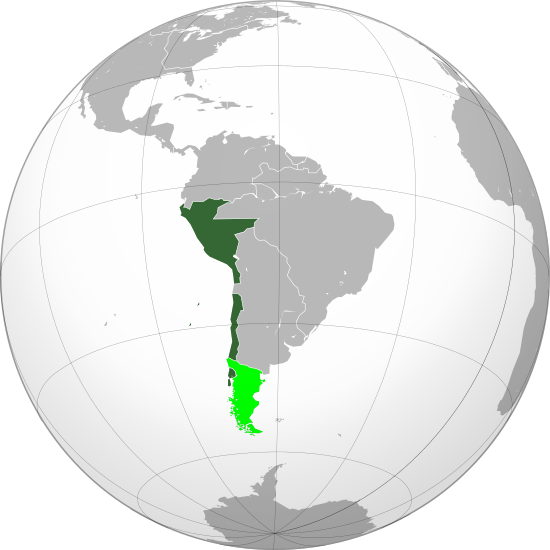
\includegraphics[width=\textwidth]{vice_peru.png}
\caption{\label{fig:1a}}
\end{subfigure}
\begin{subfigure}{0.15\textwidth}
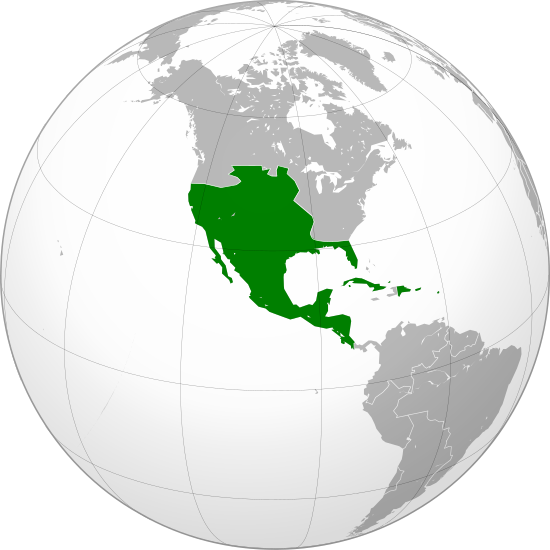
\includegraphics[width=\textwidth]{vice_nuevaespana.png}
\caption{\label{fig:1b}}
\end{subfigure}
\begin{subfigure}{0.15\textwidth}
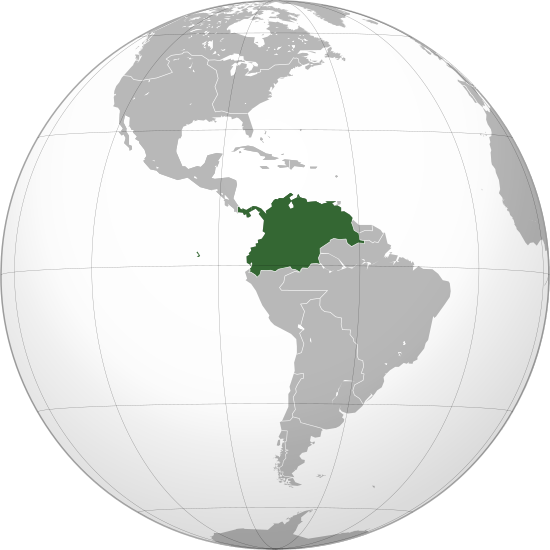
\includegraphics[width=\textwidth]{vice_nuevagranada.png}
\caption{\label{fig:1c}}
\end{subfigure}
\begin{subfigure}{0.15\textwidth}
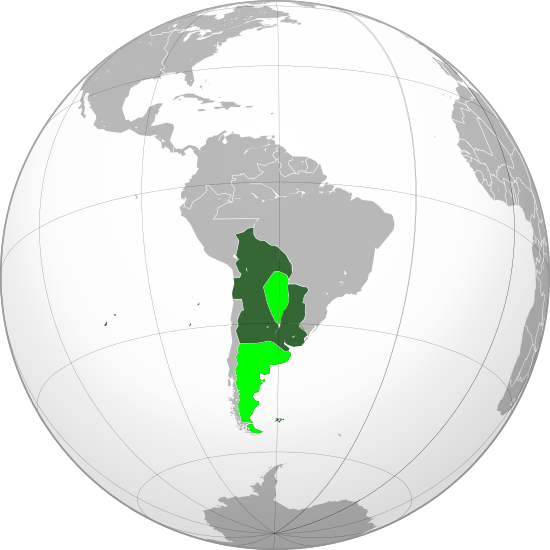
\includegraphics[width=\textwidth]{vice_riodelaplata.png}
\caption{\label{fig:1d}}
\end{subfigure}
\caption{\label{fig:1} Maps depicting \textit{virreinatos} in Latin America, 17th and 18th centuries.}
\end{figure}

\begin{enumerate}
\item Consider the maps in Fig. \ref{fig:1}.  Fill in Tab. \ref{tab:1} below.
\begin{table}[ht]
\centering
\begin{tabular}{| c | c | c |}
\hline
\textbf{Map in Fig. \ref{fig:1}} (a-d) & \textbf{\textit{Virreinato}} & Captial $~~~~~~~~~~$ \\ \hline
& \textit{Nueva Espa\~{n}a} & $~~~~~~~~~~$ \\ \hline
& \textit{Nueva Granada} & $~~~~~~~~~~$ \\ \hline
& \textit{R\'{i}o de la Plata} & $~~~~~~~~~~$ \\ \hline
& \textit{Per\'{u}} & $~~~~~~~~~~$ \\ \hline
\end{tabular}
\caption{\label{tab:1} Fill in the missing information.}
\end{table}
\item According to the author of Chapter 2, what industry is thought to be the origin of the learned societies, and later new colleges and universities, in Nueva Espa\~{n}a? Explain why.  \\ \vspace{1.5cm}
\item Discuss the importation of scientific texts and journals during the Enlightenment period to the New World.  Consider Carlos de Sig\"{u}enza y G\'{o}ngora, a Jesuit priest, mathematician, astronomer, and physicist.  What kinds of texts were found in his library? \\ \vspace{3cm}
\item Given that the Bourbons of France held the Spanish throne in the 18th century, we might expect the French Enlightenment to spread within Latin America. (a) What forces were opposed to this transmigration of ideas?  (b) How was the tension resolved? (c) Consider the Deville Brothers, and Agust\'{i}n Dherbe, vendors of scientific texts and other books. How much of their business involved exports to Spain and Mexico?  What can you say about the volume of this trade? (d) What were some of the accomplishments of Father Diego Cisneros in Lima, regarding the spread of scientific knowledge? \\ \vspace{3cm}
\item Another fascinating account of the private libraries of Latin American scientists comes from Jos\'{e} Ignacio Bartolache.  His library included books in the following languages: Latin, Greek, Hebrew, Nahuatl, English, and French.  (a) What does the distribution of texts in this library tell us about the scientific attitude of Latin Americans in the 18th Century? (b) What other scientific items did Bartolache own, and what clues does this add to our picture of the scientific attitude in that time and place?  (c) Considering these collections were built before 1760, draw a comparison to the state of science in the American colonies (later the United States).
\end{enumerate}

\end{document}
